\documentclass[a4j, 12pt]{jarticle}
\usepackage{graphicx}
\usepackage{titling}
\usepackage{amsmath}
\usepackage{float}
\usepackage{listings}
\usepackage{booktabs}
\usepackage{siunitx}

\renewcommand{\lstlistingname}{コード}
\graphicspath{{./assets/}}
\title{様々なソートアルゴリズム}
\author{クリスティアン ハルジュノ\thanks{釧路工業高等専門学校情報工学科5年情報21番}}
\date{\today}
\begin{document}
\begin{titlepage}
  \centering
  \vspace*{3cm}

  {\fontsize{25pt}{36pt}\selectfont\bfseries ソートプログラム} \\[1cm]  % Main title
  {\Large 釧路工業高等専門学校情報工学科5年・情報工学実験II} \\[1cm]
  {\large 氏名:クリスティアン・ハルジュノ} \\[1cm]
  {\large 出席番号:21} \\[1cm]
  {\large 学籍番号:234071} \\[5cm]


  {\Large 提出日:2025年6月17日} \\

  \vfill

\end{titlepage}
\section{初めに}
データに最適なソートアルゴリズムを選択するのは容易ではありません. Big-O記法を用いて理論的にアルゴリズムを比較することは可能ですが, 現実のソートアルゴリズムはそれ以上の要素を含んでいます. \\

理論的に効率的なアルゴリズムの中には, 実装前に徹底的に調査する必要がある弱点を持つものもあります. 一部のアルゴリズムは, データがアルゴリズムを最適に実行できる特定の状態にある場合にのみ効率的です. \\

現代のコンピュータは, 大容量メモリ, 高速CPU, 効率的なストレージなど, 十分なハードウェアスペックを備えていますが, 一部のアルゴリズムは高速実行のためにリソースを犠牲にしています. データサイズが小さい場合は, これは問題にならないかもしれません. しかし, ビッグデータ企業のようにデータを大規模化すると, リソースは適切に対処する必要がある非常に重要な問題になります. そのため, アルゴリズムを理論的に比較するだけでなく, 対象データセットに対してこれらのアルゴリズムをテストし, 結果を分析することが重要です. \\

本レポートでは, 実装が最もシンプルなものからより複雑なものまで, 最も普及している6つのソートアルゴリズムを検証し, 7つの固定データセットと比較します. 各データセットには, 1から50000までの整数が10万行含まれています. 各データセットは, 完全にランダム, 反転, ソート済みなど, さまざまな段階にあります. これらの比較により, 選択した6つのソートアルゴリズムの長所, 短所, および動作を検証できます. \\
\section{背景}
このセクションでは, この実験で使用した6つのソートアルゴリズムを紹介し, それぞれがどのように機能するかを説明します.
\subsection{ソートアルゴリズムを紹介}
\begin{description}
  \item[バブルソート] バブルソートは最もよく知られているソートアルゴリズムの一つです. 実装が非常に簡単であり, 少量のデータに対してはメモリ使用量が少なく, 処理も比較的高速です. この方法にはデータを最初から最後まで調べながら, 現在の数値と次の数値を比較することで機能します. 現在の数値が次の数値よりも大きい場合は, 位置を入れ替えます. このプロセスは, データが完全にソートされるまで何度も繰り返されます.\\
  \item[シェーカーソート] シェーカーソートまたはカクテルソートはバブルソートと似てるですが, シェーカーソートでは左から右に移動だけでなく逆向きにもう通過する. \\
  \item[挿入ソート] 挿入ソートは, 要素を適切な位置に直接挿入することで並べ替えを行うアルゴリズムです. 現在処理している要素を, それより前の要素と右から左に1つずつ比較し, 比較対象が現在の要素より大きければ, 右にずらします. 適切な位置が見つかったところで, 現在の要素を挿入します. \\
  \item[バケットソート] バケットソートは他方法より速度が最高と言えます. しかし, ソートの高速にはメモり使用量の増加が伴う. バケットソートでは, データを複数のバケットに分割します. 各バケットは, バブルソートや挿入ソートなどの手法を用いてソートされます. すべての要素を指定されたバケットに挿入した後, すべてのバケットを連結してソート済みの配列を作成します. この手法は, 大規模なデータに対して単純なソートアルゴリズムを実行する必要がないため, 高速です. 前述のように, バブルソートなどの一般的なソート手法は, 大規模なデータベースではパフォーマンスが低下します. しかし, 少量のデータであれば問題ありません. データを独自のバケットに分割することで, 1回の操作で処理しなければならないデータ量が大幅に削減され, アルゴリズムの負荷が軽減されます. \\
  \item[クイックソート] クイックソートは分割統治ソートと言われています. このソート方法ではある配列から枢軸を選び, 全要素をその枢軸に比較する. 枢軸より小さいとその要素を枢軸の左がわにづらす. 枢軸より大きいと, その要素を枢軸の右側にづらす. 枢軸を分岐点とし, 配列を左配列と右配列に分割する. この処理を各文割された配列に対応し, 繰り返して行う. 最小配列に着くと, 各配列をまた分岐点枢軸の左と右側に繋ぎます. \\
  \item[カウントソート] バケットソートと似たように, このソート方法でもバケットのような配列を作成する. まず, データ配列内の最大値を探索し, その値をもとにカウント配列(頻度を格納するための配列)を作成する. 次に, 元のデータ配列を1つずつ走査し, それぞれの値に対応するインデックスのカウント配列の値をインクリメントすることで, 各値の出現回数を記録する. その後, カウント配列を累積和に変換し, それをもとに元のデータを安定的に新しい配列へと並べ替えていく. このソートは整数値に限定されるが, 非高速でソートできます. \\
\end{description}

\subsection{理論的な比較}
表\ref{tab:sort-comparison}, セクション2.1で前述した各ソート手法の基本的な特性または動作を示しています. 各アルゴリズムの特性は, 最良の計算複雑度, 平均的な計算量, 最悪の計算量に分類されます. 最良の計算量は, 特定の入力状態においてデータをソートするために必要な最小の演算量を表します. 平均的な計算量は, 考えられるすべての入力を考慮し, データをソートするために必要な予想される演算量を表します. 最悪の計算量は, 特定の入力状態においてデータ処理に必要な最大の時間を表します.
\begin{table}[htbp]
  \centering
  \caption{各ソートアルゴリズムの計算量と特徴の比較}\label{tab:sort-comparison}
  \resizebox{\linewidth}{!}{%
    \begin{tabular}{|l|c|c|c|c|c|c|}
      \hline
      \textbf{アルゴリズム} & \textbf{最良計算量} & \textbf{平均計算量} & \textbf{最悪計算量} & \textbf{空間計算量} & \textbf{インプレース} \\
      \hline
      バブルソート       & $O(n)$          & $O(n^2)$         & $O(n^2)$         & $O(1)$            & はい \\
      シェーカーソート   & $O(n)$          & $O(n^2)$         & $O(n^2)$         & $O(1)$           & はい \\
      挿入ソート         & $O(n)$          & $O(n^2)$         & $O(n^2)$         & $O(1)$           & はい \\
      バケットソート     & $O(n + k)$      & $O(n + k)$       & $O(n^2)^\dagger$ & $O(n + k)$       & いいえ \\
      クイックソート     & $O(n \log n)$   & $O(n \log n)$    & $O(n^2)$         & $O(\log n)^*$   & はい \\
      カウントソート     & $O(n + k)$      & $O(n + k)$       & $O(n + k)$       & $O(k)$           & いいえ \\
      \hline
    \end{tabular}
  }
\end{table}

計算量を指定するために, Big O表記法を使用します. Big O表記法は, 処理する必要があるデータの量に基づいてソート アルゴリズムのパフォーマンスを評価する最も基本的な方法の1つです. 表\ref{tab:sort-comparison}に示されているように, バブルソート, シェイカーソート, 挿入ソートの平均計算量は$O(n^2)$です. Big O表記法では, $n$はデータ自体の長さに対応します. データのソートに必要な操作数に対して$n$をプロットすると, 計算量が$O(n^2)$の図\ref{bigograph}に示すように, ソートするデータの数がわずかに変化するだけでも操作数が大幅に増加し, 大量のデータのソート効率が低下する可能性があります. しかし, 計算量が$O(n \log n)$のクイックソートを\ref{bigograph}と比較すると, データ量を大幅に増やした場合でも, 特定のデータをソートするために必要な操作の量は, 複雑度が$O(n^2)$のアルゴリズムに比べてはるかに少なくなります.\\

上記のアルゴリズムの最良計算量について、バブルソート、シェイカーソート、挿入ソートはいずれも、与えられた入力データが既にソート済みであることを前提としています。この場合、アルゴリズムはデータを1回だけ処理すればよいため、計算量は$O(n^2)$から$O(n)$に減少します。バケットソート最良計算量では、すべての要素が各バケットに均等に分散されていると想定されます。クイックソートの最良計算量では、ピボットの選択によって値が左右に均等に分散されると想定されます。最後に、カウントソートの最良計算量では、入力データの整数の範囲が狭いと想定されます。\\

最後に, 外部配列を用いてデータの内容をソートするバケットソートとカウントソートの場合, 平均的な計算量は$O(n + k)$で測定されます. ここで, $k$は外部配列の処理に必要な演算量を表します. $k$を調整することで, 特定のデータのソートに必要な演算量を大幅に削減可能性がある.\\

\begin{figure}[H]
  \centering
  \includegraphics[width=0.8\linewidth]{bigo.eps}
  \caption{様々な計算量を比較}\label{bigograph}
\end{figure}

表\ref{tab:sort-comparison}に基づくと, 空間計算量とインプレースは, ソートが元のデータ配列自体の外で行われることを指します. バブルソート, シェイカーソート, 挿入ソートの空間計算量が$O(1)$ので, 与えられたデータをソートするために必要な空間の量は最初から変わりません. つまり, これらのアルゴリズムは非常に空間効率が高く, 元のデータとは別に新しいメモリを割り当てる必要がありません. バケットソートとカウントソートのアルゴリズムの空間計算量は$O(n + k)$と$O(k)$であり, この場合, $k$はデータをソートするために作成される新しい空間の量を指します. これらのアルゴリズムは新しい空間を割り当てる必要があり, アルゴリズムの設定方法によっては大量のメモリを消費する可能性があります. クイックソートは特に注目すべき点です. クイックソートの空間計算量は$O(\log n)$ですが, すべての操作はデータ配列内で行われ, 新しいメモリを割り当てる必要はありません. そのため, クイックソートはインプレースソートアルゴリズムと呼ばれます. クイックソートはソートが進むにつれて, 処理が必要なデータの長さが縮小し続けるためです.\\

\section{実験セットアップ}
\subsection{ハードウェアと環境}
ハードウェアとしてはAppleシリコンのプロセッサに基づいて実験を行います。
\begin{description}
  \item[機種名] Apple Macbook Pro (M3, 2023年モデル)
  \item[プロセッサ] Apple M3チップ(8コア:高性能コア4+高効率コア4)
  \item[GPU] 10コア統合型GPU
  \item[メモリ] 16GBユニファイドメモリ
  \item[ストレージ] 1TB SSD
  \item[OS] macOS Sequoia 15.5
  \item[アーキテクチャ] ARM64(Appleシリコン) 
\end{description}
また、作成した実験プログラムはC言語で書き、GCCコンパイラでコンパイルされます。
\begin{verbatim}
  Apple clang version 17.0.0 (clang-1700.0.13.5)
  Target: arm64-apple-darwin24.5.0
  Thread model: posix
\end{verbatim}
コンパイルを効率化するため、GCCコンパイラをMakeと同時に利用します。
\begin{verbatim}
  GNU Make 3.81
  Copyright (C) 2006  Free Software Foundation, Inc.
  This is free software; see the source for copying conditions.
  There is NO warranty; not even for MERCHANTABILITY or 
  FITNESS FOR A PARTICULAR PURPOSE.
  This program built for i386-apple-darwin11.3.0
\end{verbatim}
\subsection{実験に使用するデータセット}
各ソート アルゴリズムの制限と動作を適切にテストするために、1 から 50000 までの範囲の 100000 個の整数を含む 7 つのデータセットを用意しました。各データセットの構造は、適用されたソート アルゴリズムの動作を引き出すためにさまざまな方法で配置されています。
\begin{table}[htbp]
  \centering
  \caption{各データファイルの内容}
  \begin{tabular}{|c|c|c|}
    \hline
    ファイル名 & データ数 & データの種類 \\
    \hline
    data1.dat & 100,000 & ランダムデータ \\
    data2.dat & 100,000 & ランダムデータ \\
    data3.dat & 100,000 & ランダムデータ \\
    data4.dat & 100,000 & 昇順データ \\
    data5.dat & 100,000 & 降順データ \\
    data6.dat & 100,000 & バイトニックデータ \\
    data7.dat & 100,000 & ジグザグデータ \\
    \hline
  \end{tabular}\label{tab:dataset-summary}
\end{table}
表2を見ると、データセット1から3にはすべて10万個の整数が含まれており、それらはランダムに並べられていることがわかります。データセット4には、適用されたアルゴリズムの最良のシナリオをシミュレートするために既にソートされたデータが含まれています。データセット5は、ソートアルゴリズムの最悪のシナリオをシミュレートするために、逆順にソートされています。\\

データセット6はバイトニックシーケンスで配置されています。数式\ref{bitonicsequence}により、バイトニックシーケンスとは、データセットの先頭から緩やかに上昇し、中央でピークに達し、その後、データセットの末尾に近づくにつれて緩やかに下降するデータと説明できます。\\
\begin{equation}\label{bitonicsequence}
a_1 < a_2 < \cdots < a_k > a_{k+1} > \cdots > a_n
\quad (1 \leq k < n)
\end{equation}

データせっと6の先頭付近と中間付近と末尾付近からサンプル要素をランダム的に取って、表\ref{tab:data6-sample}のようになります。
\begin{table}[H]
  \centering
  \caption{バイトニックデータ(data6.dat)のサンプル値}
  \begin{tabular}{|c|c|}
    \hline
    位置 & サンプル値(例) \\
    \hline
    先頭付近 & 17131, 41279, 23264, 44242, 2505, 6637, 5374,\\
    中間付近(最大付近) & 43248, 43247, 43247, 43246, 43244 \\
    末尾付近 & 12, 12, 10, 10, 9, 9, 9, 9, 8, 8, 7, 5, 2 \\
    \hline
  \end{tabular}\label{tab:data6-sample}
\end{table}

データセット7はジグザグ配列になっています。数式\ref{tab:data7-sample}ジグザグ配列とは、データ全体を通して小さな数値と大きな数値が交互に現れるデータのことです。この場合、データセットはランダム化され、「小さい」部分と「大きい」部分が交互に現れます。データセットは、これらの大きな部分と小さな部分が、長さを変えながら交互に現れます。\\
\begin{equation}\label{zigzagsequence}
  a_1 < a_2 > a_3 < a_4 > a_5 < \cdots
\end{equation}
データせっと7の先頭付近と中間付近と末尾付近からサンプル要素をランダム的に取って、表\ref{tab:data6-sample}のようになります。
\begin{table}[H]
  \centering
  \caption{ザクザクデータ(data7.dat)のサンプル値}
  \begin{tabular}{|c|c|}
    \hline
    位置 & サンプル値(例) \\
    \hline
    先頭付近 & 2, 2, 2, 4, 7, 7, 7, 8, 13, 15 \\
    中間付近 & 20778, 42992, 29869, 31747, 22945, 40054, 38945, 47166 \\
    末尾付近 & 11990, 7746, 38998, 35057, 41719, 22808, 23284, 2525\\
    \hline
  \end{tabular}\label{tab:data7-sample}
\end{table}
\subsection{測定について}
ソートアルゴリズムの実行時間を正確に測定するために、C言語の$time.c$ライブラリを利用します。$time.c$ライブラリには、プログラム実行後に経過したCPUティック数を測定する$clock()$関数が用意されています。図\ref{fig:clockcode}により、$clock()$関数を使用することで、ソート関数の実行前から完了後までのティック数を測定します。得られたティック数を、CPUが1ティックを実行するのにかかる時間で割ります。この値を計算すると、ソート関数の合計実行時間が算出されます。
\begin{figure}[htbp]
  \centering
  \caption{プログラムの測定分の例}\label{fig:clockcode}
  \begin{lstlisting}[basicstyle=\ttfamily\small]
    start_time = clock();
    shakerSort(fileLength, clonedArray);
    end_time = clock();
    elapsed_time = (double)(end_time - start_time)
                    /CLOCKS_PER_SEC;
  \end{lstlisting}
\end{figure}
\newpage
\subsection{各アルゴリズムの説明}
\subsubsection{バブルソート}
\begin{enumerate}
  \item リストの最初の位置から始める. 
  \item 現在の数値と次の数値を比較する. 
  \item 現在の数値が次の数値より大きければ, 入れ替える. 
  \item 次の位置に進み, リストの末尾までステップ2〜3を繰り返す. 
  \begin{figure}[H]
    \centering
    \includegraphics[width=0.8\linewidth]{bubble1.eps}
    \caption{先頭から末尾まで数値を比較して, 交換する. }
  \end{figure}
  \item 1回の通過が終わったら, 最初の位置に戻って再び通過を行う. 
  \begin{figure}[H]
    \centering
    \includegraphics[width=0.8\linewidth]{bubble2.eps}
    \caption{通過後最初の位置に戻って, 再び通過}
  \end{figure}
  \item 通過中に1回も入れ替えがなければ, ソートは完了. 
  \item 入れ替えがあった場合, ステップ1〜6を繰り返す. 
  \begin{figure}[H]
    \centering
    \includegraphics[width=0.8\linewidth]{bubble3.eps}
    \caption{通過後に入れ替えされた要素がないと終了}
  \end{figure}
\end{enumerate}
\subsubsection{シェーカーソート}
\begin{enumerate}
  \item 配列の先頭から走査を開始する. 
  \item 現在の要素と次の要素を比較し, 現在の要素の方が大きければ交換する. 
  \item 配列の末尾まで進み, 走査中に交換が一度も行われなければソートを終了する. 
  \item 次に逆方向(末尾から先頭)に走査する. 
  \item 現在の要素と前の要素を比較し, 現在の要素の方が小さければ交換する. 
  \item 先頭まで進み, 走査中に交換が一度も行われなければソートを終了する. 
  \item 上記の操作を, 交換が行われる限り繰り返す. 各往復ごとに走査範囲を狭めることができる. 
  \begin{figure}[H]
    \centering
    \includegraphics[width=0.8\linewidth]{shaker.eps}
    \caption{シェーカーソートの進み方}
  \end{figure}
\end{enumerate}
\newpage
\subsubsection{挿入ソート}
\begin{enumerate}
  \item 最初の要素をソート済み部分とみなす. 
  \item 次の要素を取り出して, ソート済み部分の各要素と比較する. 
  \item ソート済み部分の中で, 自分より大きい要素を右にずらす. 適切な位置に挿入する. 
  \item 適切位置がないとそのままで次の位置に進む
  \begin{figure}[H]
    \centering
    \includegraphics[width=\linewidth]{insertion1.eps}
    \caption{第二位置からスタート. ソート済み要素より大きい数値を左にずらす.}
  \end{figure}
  \item リストの末尾までステップ2〜4を繰り返す. 
  \item ソートされていない要素がないと終了
  \begin{figure}[H]
    \centering
    \includegraphics[width=\linewidth]{insertion2.eps}
    \caption{ソート対象値がないとソート終了}
  \end{figure}
\end{enumerate}
\subsubsection{バケットソート}
作成するバケット数の選択は、再現性を確保し、パフォーマンス評価の一貫性を維持するために重要であるため、入力特性に基づいて動的に決定するのではなく、すべてのテスト実行でバケット数を固定しました。本レポートの結果の大部分では、バケット数を100としています。また、バケット数がメモリ使用量とソート速度に与える影響についても考察します。\cite{gfg:bucketsort2024}\\
\begin{enumerate}
  \begin{figure}[H]
    \centering
    \includegraphics[width=\linewidth]{bucket1.eps}
    \caption{ソート対象データ}
  \end{figure}
  \item 最初に、ソート対象の整数の範囲(例:0〜2.5)を確認し、その範囲に応じてバケットの数を決める(例:3の範囲ごとにバケットを作成するなど)。
  \begin{figure}[H]
    \centering
    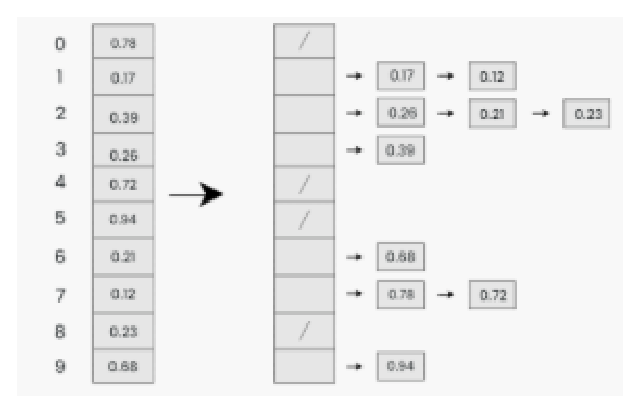
\includegraphics[width=0.8\linewidth]{bucket2.eps}
    \caption{作成したバケット}
  \end{figure}
  \item 各要素をその値に基づいて対応するバケットに振り分ける。
  \begin{figure}[H]
    \centering
    \includegraphics[width=0.8\linewidth]{bucket3.eps}
    \caption{適当に作成されたバケットに要素を入れる。}
  \end{figure}
  \newpage
  \item 各バケット内の要素をソートする(挿入ソートやバブルソートなど、単純なソートでOK)。
  \begin{figure}[H]
    \centering
    \includegraphics[width=0.8\linewidth]{bucket4.eps}
    \caption{各バケットの内容をソートし、連続}
  \end{figure}
  \item すべてのバケットを順番に結合して、最終的なソート済み配列を作る。
  \begin{figure}[H]
    \centering
    \includegraphics[width=0.8\linewidth]{bucket5.eps}
    \caption{ソートずみの配列}
  \end{figure}
\end{enumerate}
\subsubsection{クイックソート}
クイックソートを利用する場合、ピボットポイントの選択はアルゴリズムのパフォーマンスに重要です。最適なピボットポイントは、小さい(左)配列と大きい(右)配列を均等に分割できるものです。常に最大のピボット値または最小のピボット値を選択すると、すべてのデータ値をピボットポイントの左側または右側に移動する必要があるため、ソートアルゴリズムの効率が大幅に低下します。その結果、計算量は$O(nlogn)$から$O(n^2)$に変化します\cite{gfg:quicksort2025}。\\
\begin{enumerate}
  \item 初めに、配列から枢軸(ピボット)を1つ選びます。選び方には、先頭、中央、末尾などさまざまな方法があります。
  \item 配列の各要素を枢軸と比較し、小さい要素は枢軸の左側、大きい要素は右側に移動させます(パーティショニング)。
  \item 枢軸を基準にして、配列を左側部分(枢軸より小さい要素)と右側部分(枢軸より大きい要素)に分割します。
  \item 左右それぞれの部分配列に対して、同様にステップ1~3を再帰的に繰り返します。
  \begin{figure}[H]
    \centering
    \includegraphics[width=\linewidth]{quick1.eps}
    \caption{枢軸を選び、左側分と右側分に分割します。左と右配列を再帰的に処分}
  \end{figure}
  \item 各部分配列の要素数が1以下になると、すべての部分配列が整列され、結果的に全体がソートされます。
  \begin{figure}[H]
    \centering
    \includegraphics[width=0.8\linewidth]{quick3.eps}
    \caption{部分配列を整列され、結果的に全体がソートされます}
  \end{figure}
\end{enumerate}
\subsubsection{カウントソート}
\newpage
\section{実験結果}
\subsection{データセットごとに実行}
各ソートアルゴリズムのパフォーマンスを各テストケース(データセット)に対して比較するために、すべてのアルゴリズムを単一のデータセットに対して実行するソートプログラムを実行します。\\
ハードウェアメーカーによって実装された低レベルの最適化とハードウェア効果により、CPUはプログラムの次の実行部分を予測または推測し、繰り返し実行されるシステムコールを高速化するために最適化することができます\cite{mittal2018branch}。CPUはまた、最初の実行時にこのデータセットをRAMにロードします。アルゴリズムが繰り返し実行されると、ロードされたデータセットはCPUダイ自体のより高速なキャッシュにゆっくりと移動され、メモリアクセスのレイテンシが大幅に低減されます\cite{apple2023siliconcpuopt}。表\ref{repeatedsortresult}により、これらの最適化のせいで、単一のソートアルゴリズムを繰り返し実行すると、時間の経過とともに結果が徐々に高速化され、結果の不正確さが生じます。この問題を軽減するために、各アルゴリズムを10回実行し、結果を平均します。
\begin{table}[H]
  \centering
  \caption{ソートアルゴリズムを10回繰り返して実行する場合}\label{repeatedsortresult}
  \begin{tabular}{|l|l|r|r|r|}
    \hline
    \textbf{File Name} & \textbf{Sort Method} & \textbf{Data Length} & \textbf{Time(sec)} & \textbf{Memory (KB)} \\
    \hline
    data1.dat & Counting Sort & 100000 & 0.000803 & 400.00 \\
    data1.dat & Counting Sort & 100000 & 0.000804 & 400.00 \\
    data1.dat & Counting Sort & 100000 & 0.000805 & 400.00 \\
    data1.dat & Counting Sort & 100000 & 0.000808 & 400.00 \\
    data1.dat & Counting Sort & 100000 & 0.000790 & 400.00 \\
    data1.dat & Counting Sort & 100000 & 0.000762 & 400.00 \\
    data1.dat & Counting Sort & 100000 & 0.000741 & 400.00 \\
    data1.dat & Counting Sort & 100000 & 0.000736 & 400.00 \\
    data1.dat & Counting Sort & 100000 & 0.000736 & 400.00 \\
    data1.dat & Counting Sort & 100000 & 0.000763 & 400.00 \\
    \hline
  \end{tabular}
\end{table}

\subsubsection{データセット1に対する実行結果}
\begin{table}[H]
  \centering
  \caption{各ソートアルゴリズムの\texttt{data1.dat}に対する実行結果}
  \resizebox{\textwidth}{!}{%
    \begin{tabular}{|l|l|r|r|r|}
      \hline
      \textbf{File Name} & \textbf{Sort Method} & \textbf{Data Length} & \textbf{Time Avg (sec)} & \textbf{Memory (KB)} \\
      \hline
      data1.dat & Counting Sort  & 100000 & 0.000815  & 600.00  \\
      data1.dat & Bucket Sort    & 100000 & 0.003011  & 1084.88 \\
      data1.dat & Quick Sort     & 100000 & 0.008440  & 400.00  \\
      data1.dat & Insertion Sort & 100000 & 3.066381  & 400.00  \\
      data1.dat & Shaker Sort    & 100000 & 12.019590 & 400.00  \\
      data1.dat & Bubble Sort    & 100000 & 16.944878 & 400.00  \\
      \hline
    \end{tabular}%
  }
\end{table}
\section{分析と議論}
\section{まとめ}
\section{発表について}

\bibliographystyle{plain}
\bibliography{references}

\end{document}